\documentclass[conference]{IEEEtran}
\IEEEoverridecommandlockouts
% The preceding line is only needed to identify funding in the first footnote. If that is unneeded, please comment it out.
\usepackage{cite}
\usepackage{amsmath,amssymb,amsfonts}
\usepackage[utf8]{inputenc}
\usepackage{algorithmic}
\usepackage{graphicx}
\usepackage{textcomp}
\usepackage{xcolor}
\graphicspath{{Images/}} 
%\def\BibTeX{{\rm B\kern-.05em{\sc i\kern-.025em b}\kern-.08em
 %   T\kern-.1667em\lower.7ex\hbox{E}\kern-.125emX}}
\begin{document}

\title{Mehrwert der rollenbasierten Umsetzung von kollaborativen Lernumgebungen\\}


\author{\IEEEauthorblockN{Hung Tran Duc}
\IEEEauthorblockA{\textit{Technische Universität Dresden} \\
Dresden, Deutschland \\
hung.tduc@yahoo.com}
}



\maketitle

\begin{abstract} Rollenbasierte Sprachen werden seit Jahrzehnten als Alternative zu objektorientierten Ansätzen untersucht. Die Natur der Rolle erlaubt es Obbjekten, sich dynamisch and verschiedene Anforderungen anzupassen. Mit zunehmend komplexer und offener Software, besteht eine wachsende Nachfrage nach adaptiven Systemen. Kollaborative Lernumgebungen fördern je nach Anwendung die Sozialkompetenz, Eigeninitiative oder Konzentrationsfähigkeit der Lernenden. In dieser Arbeit soll beleuchtet werden, welche Vorzüge eine Lernumgebung auf der Grundlage von Rollen aufweist.
\end{abstract}

\begin{IEEEkeywords}
kollaborative Lernumgebung, e-Learning, rollenbasiert
\end{IEEEkeywords}

\section{Einleitung}
% Motivation Rollen: - RML seit Jahrzehnten untersucht -> Potenzial (Bachman) \cite{bachman} - Breite an Bereichen: Datenmodelle, Konzeptmodelle, Programmiersprache (Loebe 2005 ; Guarino und welty 2009, Halpin 2005; Hennicker 2015) - Aktuelle Software: zunehmend komplex und Kontextabhängig(offen,verteilt) -> Nachfrage nach OOP-Alternativen
% Motivation, warum ich von rollen erzähle: alternative zu oom, lang und breit untersucht, potenzial, aktuelle Nachfrage
%oom ist dominierend, trotzdem lohnt es sich alternativen zu überlegen für innovative systeme, welche möglichkeiten aufzeigen könnten, welche mit OO noch nicht erkenntlich waren
Objektorientierte Programmierung ist das verbreiteste und am häufigsten angewendete Programmierparadigma. Dennoch kann es sich lohnen, Alternativen zu untersuchen. Sie könnten zu innovativen Konzepten führen, welche Mittel und Wege aufzeigen, die mit Objektorientierung nicht erkenntlich waren. Beispielalternativen sind funktionsorientierte Programmierung, welche sich auf die Modellierung von Prozessen fokusierte, oder aspektorientierte Programmierung. Letztere bietet die Möglichkeit zentral Verhalten, das mehrere unabhängige Klassen annehmen müssen, zu definieren. \\ Rollenbasierte Programmierung stellt eine weitere Alternative zur Objektorientierung dar. Zum ersten Mal wurden Rollen 1977 von Bachman et al. charakterisiert. Sie beschreiben Rollen als festgelegtes Verhalten, welches von Objekten verschiedener Klassen angenommen werden kann \cite{bachman}. Seitdem wurde der Begriff der Rolle stets wieder aufgegriffen und in verschiedenen Bereichen thematisiert. Diese Bereiche umfassen Ontologien\cite{loebe2005abstract}\cite{guarino2009overview}, Datenmodellierung \cite{halpin2005orm}, Konzeptmodellierung \cite{hennicker2015model} und Programmiersprachen \cite{ubayashi2000roleep}. In \cite{steimann2000representation} hat Steimann aktuelle Untersuchungen zu Rollen zusammengefasst und bewertete den Einfluss der Rolle auf die moderne Datenmodellierung als gering. Diese Beobachtung und die Menge an Untersuchungen, sowohl vor als auch nach Steimann, weisen auf ein großes aber ungenutztes Potenzial der Rolle als Programmierparadigma hin. Eine Rolle beschreibt Attribute und Verhalten von Objekten, die in einem bestimmten Kontext miteinander kollaborieren. Ein Objekt kann also je nach Bedarf eine neue Rolle und somit auch neues Verhalten annehmen. Diese Anpassungsfähigkeit kann behilflich sein, da moderne Softwaresysteme zunehmend komplexer und offener werden \cite{murer2008managed}. \\
%Motivation  Collab E-Learning:- Eigenverantwortung und Initiative- gemeinsamer austausch- höhere motivation durch gruppengefühl, - ausprägung sozialkompetenz- voranschreitende digitalisierung (VON ALLEM) 
% Motivation für kollaborative Lernumgebungen: was sind sie/neu, wachsend -> Potenzial, verbreitung(Arten,beispiele), vorteile: gruppengefühl, aufmerksamkeit, eigeninitiative, globalität, 
In den meisten Hochschulen werden mittlerweile Lernplattformen verwendet. Neben der Bereitstellung von Lehrmaterialien, dienen sie auch zur Organisation von Lernvorgängen. Als Lernumgebung erleichtern sie den Lernenden die Kommunikation untereinander oder mit den Vortragenden. Der Lernprozess kann somit zu beliebiger Zeit an einem beliebigen Ort mit einem mobilen Endgerät durchgeführt werden. Audience Response Systeme (ARS) werden während Lehrveranstaltungen eingesetzt. Sie ermöglichen es, von allen Zuhörern gleichzeitig Feedback bzw. Input einzuholen.Browserbasiert oder als mobile App verfügbar , benötigen die Systeme keine spezielle Hardware. Primärer Anwendungsfall ist das Stellen von Fachfragen um den Vorbereitungsgrad oder den Lernstand des Publikums zu ermitteln. Es konnte beobachtet, dass das ARS zu einem deutlich höherem Engagement in Vorlesungen führt. Zusätzlich konnten bei Studenten eine kontinuierliche Aufmerksamkeit und höhere Lernleistung festgestellt werden \cite{digitaleHochschule}. Eine andere Anwendung stellen kollaborative Lernumgebungen dar. Sie haben ein einfaches Grundprinzip: Lernende werden in Gruppen geteilt um gemeinsam Aufgaben zu lösen. Sie teilen die Aufgaben untereinander auf und tauschen ihre Kenntnisse aus. Auf diese Weise werden Sozialkompetenz und Organisationsfähigkeit gefördert. Auch die Motivation eines Studierenden, kann durch das Gefühl der Gruppenzugehörigkeit gesteigert werden. Der Fokus auf Kollaboration, sowie die verschiedenen Anwendungsfälle legen nahe, dass Lernumgebungen aus einer rollenbasierten Umsetzung einen Vorteil ziehen könnten. \\ In dieser Arbeit wird diskutiert, welche Vorzüge eine rollenbasierte Lernumgebung gegenüber einer klassisch objektorientierten Umsetzung haben könnte. Dazu wird in Kapitel II eine frühere Arbeit, die sich mit rollenbasierten kollaborativen Umgebungen beschäftigte, zusammengefasst. Im darauffolgendem Kapitel III werden zuerst Anforderungen, in Form verschiedener Szenarien in Kollaborativen Lernumgebungen, beschrieben. Nachfolgend wird auf die Herausforderungen und Grenzen der objektorientierten Programmierung eingegangen. Kapitel IV beschäftigt sich mit dem Konzept der Rolle und verschiedenen Ansichten. Anschließend werden im Kapitel V die Hindernisse bei der Arbeit mit Rollen erklärt. Kapite VI beschreibt die Umsetzung einer kollaborativen Lernumgebung in ein Modell und in Kapitel VII werden die Erkenntnisse dieser Arbeit zusammengefasst.


%wie wichtig roles für collaboration sind, großes problem: rollen klar definieren und dabei flexibel bleiben, schließt oft einander aus, klärt rollenbegriff,  bewertet anwendung von rollen in collabs, nennt nötige prinzipien und mechanismen, schlussfolgerung: rollen brauchen mehr aufmerksamkeit
\begin{figure}
\label{fig:roleWrapper}
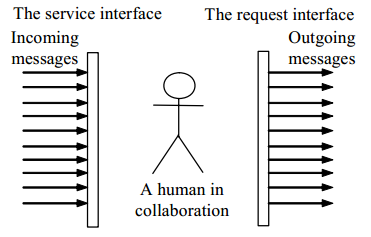
\includegraphics[scale = 0.8]{Images/roleWrapper.PNG}
\caption{Eine Rolle unterstützt als Wrapper in einer kollaborativen Umgebung die Kommunikation zwischen Mensch und Computer. \cite{zhu2006role}}
\end{figure}
\section{Verwandte Arbeiten} Zhu evaluierte die Umsetzung der Rolle in computergestützten Kollaborationssystemen\cite{zhu2006role}. Und befand, dass in den meisten damaligen Systemen die Rolle lediglich als Label für Objekte benutzt wurde. Oft wurde in einer ,,Switch/Case"-Struktur festgelegt, welche Rolle, welches Verhalten auslöst. Waren die Umgebung und die enthaltenen Rollen einmal implementiert, war es sehr aufwendig, an den Rollen Anpassungen vorzunehmen.\\ In kollaborativen Umgebungen, steht die Zusammenarbeit bzw. der Austausch zwischen Nutzern im Vordergrund. Auf Grundlage dieser Ansicht, stellt Zhu die Behauptung auf, es gäbe lediglich zwei Existenzzustände eines Objektes. Der \textit{Client} formuliert und sendet Anweisungen, während der \textit{Server} eingehende Anfragen abarbeitet. Eine Rolle würde vorgeben, was Nutzer und Umgebung bei einem bestimmten Kontext voneinander erwarten bzw fordern. Durch das Annehmen einer Rolle, erhält der Nutzer spezielle Rechte, oder auch Verpflichtungen. Eine Rolle stellt im kollaborativen System einen Wrapper dar, der ein Objekt ,,ummantelt" und ihm neue Eigenschaften verleiht (Siehe Abb.1). Der Wrapper besteht aus zwei Teilen: Die Schnittstelle für ausgehende Nachrichten, welche Anfragen an das System sendet, und eine Schnittstelle für eingehende Nachrichten, um die Anfragen anderer Objekte zu verarbeiten. \\ Desweiteren formulierte Zhu mehrere Grundprinzipien für den Aufbau eines Kollaborativen Systems. Das System ist dazu gedacht die Zusammenarbeit von Menschen zu erleichtern, egal ob sie sich am selben Ort befinden oder nicht. Die Grundprinzipien beschreiben die Eigenschaften der Objekte, Rollen und Gruppen. Zusammengefasst loggen sich Nutzer beispielsweise über einen Internetbrowser in das System ein, werden durch ein \textit{Agentenobjekt} repräsentiert und bekommen jeweils eine voreingestellte Gruppe und eine Rolle zugewiesen. Rollen, Klassen und Gruppen werden vom Nutzer erstellt und verwaltet. Eine Gruppe wird spezifiziert durch die Rollen, die angenommen werden müssen und weiteren Eigenschaften wie Sichtbarkeit und Zugänglichkeit. Die Rollen sind Objekte und somit Instanzen einer Klasse von Rollen. Jede Rolle gibt dem Nutzer vordefinierte Nachrichtenvorlagen, welche dazu genutzt werden, Nachrichten zwischen dem Nutzer und dem System auszutauschen. Sie kann von mehreren Nutzern gleichzeitig gespielt werden, aber ein Nutzer kann zu jedem Zeitpunkt nur eine Rolle tragen. Ist ein Nutzer nicht angemeldet, wird er durch einen Agenten vertreten, der eingehende Nachrichten sammelt und für den Nutzer bereithält.\\ Abschließend betont Zhu wie fundamental das Konzept der Rolle für kollaborative Systeme sei. Weitere Forschung würde in diversen Bereichen Fortschritte, vorteilhaft für Kollaboration, hervorbringen.


\section{Herausfoderungen einer objektorientierten Lernumgebung}
In diesem Kapitel wird eine beispielhafte kollaborative Lernumgebung für eine Hochschule beschrieben. Es werden Anwendungsfälle und die zugehörigen relevanten Vorgänge genannt. \\
Ziel ist es, eine Menge von Kontexten, Beziehungen und Interaktionen zu bilden. Zuletzt werden die Probleme einer objektorientierten kollaborativen Lernumgebung erläutert.

\subsection{Anforderungen Kollaborativer Lernumgebungen} 
Alle Studierende einer Hochschule besitzen einen Login für die Lernumgebung und sind als ,,Studierende" gekennzeichnet. Professoren, wissenschaftliche Mitarbeiter und andere Angestellte der Hochschule sind unter ,,Mitarbeiter" zusammengefasst und haben ebenfalls eigene Logindaten.
 \paragraph{Audience Response System(ARS)} Das bereits genannte ARS ist ein System um in Vorlesungen simultan von allen Hörern Input einzuholen, beispielsweise um Fachfragen zu beantworten. Diese Fachfragen und die dazugehörigen Antwortmöglichkeiten müssen vorher vom Vortragenden formuliert und im System gespeichert worden sein. Um diese Fragen jederzeit schnell aufrufen zu können, ist eine Zuordnung zur jeweiligen Lehrveranstaltung nötig, möglicherweise in Form eines Katalogs. Es besteht die Möglichkeit, dass ein Mitarbeiter mehrere Kurse leitet, in anderen Kursen als Vortragender erscheint oder die Rolle des Hörers annimmt um selbst teilzunehmen. Ein Kurs kann mehrere wechselnde Vortragende haben. Das Recht, diese Rolle zu übertragen liegt beim Kursleiter, dem Mitarbeiter, der für diesen Kurs verantwortlich ist.\\ In Seminaren oder ähnlichen Lehrveranstaltung, muss es möglich sein, die Rolle des Vortragenden für einen begrenzten Zeitraum zu übertragen. In dieser Zeit kann der neue Vortragende ebenfalls fachbezogene Fragen stellen und sich Feedback vom Publikum einholen. Die Annahme der Rolle geschieht nur während der Lehrveranstaltung. Die Formulierung der Fragen samt Antworten findet während der Vorbereitung des Vortrags statt. 
\paragraph{Arbeitsgruppen} Im Rahmen einer Lehrveranstaltung wurden Studierende in Gruppen eingeteilt. In diesen Gruppen sollen sie nun gemeinsam verschiedene Aufgaben lösen. In \cite{dewiyanti2007students} befragte Biasutti Studierende zu ihren Eindrücken, nachdem diese in einer kollaborativen Lernumgebung asynchron eine Aufgabe bearbeiteten. Als Kritikpunkte wurde, neben ungleichmäßiger Beteiligung, die Organisation innerhalb der Gruppe genannt. Eine klare Aufgabenverteilung wurde als wünschenswert betrachtet. Beispielsweise wurde von einem Probanden eine Art Sekretär der Gruppe vorgeschlagen. Der Sekretär, oder auch Koordinator, ist verantwortlich für die Organisation der Gruppe. In \cite{paechter2010students} und \cite{casamayor2009intelligent} wird betont wie wichtig es sei, dass einerseits ein Ansprechpartner zur Verfügung steht und dass  andererseits die Aktivitäten der Gruppe zum Teil überwacht werden. Casamayor et al. stellen den Ansatz vor, relevante Statistiken einer Gruppe aufzuzeichnen und bei bestimmten Ereignissen den Kursleiter zu benachrichtigen \cite{casamayor2009intelligent}. 
\paragraph{Offenes Forum} In OPAL\footnote{https://bildungsportal.sachsen.de/opal/} können zu Lehrveranstaltungen offene Foren eröffnet werden. Der Kursleiter kann durch einen Eintrag alle Studierenden über neue Informationen in Kenntnis setzen. Studierende haben die Gelegenheit Fragen zur Veranstaltung oder zu Aufgaben zu stellen, welche von anderen Studierenden oder vom Lehrer beantwortet werden kann. Jeder, der ein Thema eröffnet oder eine Antwort geschrieben hat, erhält eine Benachrichtigung bei neuen Antworten. 
\paragraph{Reviews} Enthält eine Lehrveranstaltung eine schriftliche Ausarbeitung, kann jedem Studierenden die Arbeit eines anderen zur Bewertung zugewiesen werden. Selbstverständlich können auch Kursleiter die Ausarbeitungen bewerten. 
	


%- experiences: 
%	- Orga und aufgabenverteilung
%	- Koordinator erwünscht
%	- mehr gruppengefühl erwünscht
%	- ungleichmäßige beteiligung
%- Pitfalls	
%	- Soziale interaktion nicht immer gewährleistet
%	- soziale interaktion oft auf sehr unpersönlicher ebene
%- intelligence assistant(asynchronous communication):
%	- Notwendigkeit eines "Lehrers" der bei Problemen in Gruppen eingreift
%		- TriggerProbleme: Passive Studenten, atypische Teilnahme, gruppen schaffen gar keine tasks, content von Material von niemandem gelesen, keine diskussion begonnen.
%- Tasks/Kontexte  
%	- Lehrer und Lernender
%	- Koordinator einer Gruppe
%	- Gruppe suchen
%	- Überwacher / Ansprechpartner
%	- Kursleiter auf Abruf/Bereitschaft
%	- reviewer/reviewee
%Entitäten: Student, Professor, Wissenschaftlicher Mitarbeiter
	

	
\subsection{Probleme der Umsetzung in objektorientierter Programmierung}  
%Nachteile von oom: Etabliert weil mindmodel Reenskaug, aber nur struktur, kein verhalten/kollaboration/dynamische änderung Steimann, state dependance/multi classes/supplier customer problem an kollaborativen Umgebungen -> Grafik
So etabliert und verbreitet objektorientierte Programmierung auch sein mag, so hat sie dennoch ihre Grenzen. Laut Reenskaug et al. entstand objektorientiertes Design mit dem Ziel, dass der Programmcode möglichst genau dem mentalem Modell des Endnutzers entspricht \cite{reenskaug2009dci}. Ein Nutzer soll beim Bedienen der Nutzerschnittstelle eine konkrete Vorstellung damit haben, wie er mit den Objekten des Programms interagiert. Je genauer ein Programm die Veränderungen an inneren Zuständen durch den Nutzer wiedergibt, desto intuitiver die Handhabung. Er kann nicht die tatsächlichen Vorgänge beobachten. Er braucht lediglich eine Repräsentation des Programmzustands um es zu bedienen. Diese Abbildung der Vorstellung des Users auf den Code gelingt nicht überall. Klassische objektorientierte Programmierung bietet keine Möglichkeit, die Kollaboration zwischen Objekten zu beschreiben. Algorithmen, die durch Kollaborationen erfüllt werden, und Relationen haben wie Objekte eine Struktur, die sich im Quellcode nur umständlich repräsentieren lässt. \\Steimanns Veranschaulichung der Problematik soll im Folgenden auf eine kollaborative Lernumgebung mit den oben genannten Merkmalen übertragen werden\cite{steimann2000representation}.\paragraph{Multiple, dynamische Klassifizierung} Sowohl Mitarbeiter, als auch Studierende können während der Laufzeit verschiedene Rollen annehmen und wieder ablegen, wie in Abbildung 2 veranschaulicht. Da es unmöglich ist,  vorherzusehen, wer welche Rolle spielen wird, muss ein Objekt in der Lage sein dynamisch seine Klasse zu wechseln. \paragraph{Rollen als Unterklassen} Ein \textit{Studierender} kann gleichzeitig Hörer in einem als auch Vortragender im anderen Kurs sein. Dies würde bedeuten, dass \textit{Hörer} und \textit{Vortragender} Unterklassen von \textit{Studierender} sind. Dasselbe Verhältnis besteht bei \textit{Mitarbeiter}, die ebenfalls Hörer und Vortragende sein können. Bei einer Unterklasse von sowohl \textit{Studierende} als auch \textit{Mitarbeiter} beschränkt sich das Verhalten auf die Schnittmenge der beiden Oberklassen und fällt damit klein oder leer aus.\paragraph{Rollen als Oberklassen} Hörer und Vortragender würden Oberklassen für sowohl Mitarbeiter, als auch Studierende darstellen. Das würde bedeuten, dass jeder Mitarbeiter oder Studierender ein Hörer, Vortragender oder beides ist. Es wäre nicht möglich weder Hörer noch Vortragender zu sein. \paragraph{Statusabhängigkeit} Eine Rolle als Ober- oder Unterklasse zu implementieren, führt dazu, dass ein Objekt und dessen Rollen, als eine einzelne Instanz dargestellt werden. Diese Instanz kann nur einen Status haben. Sollte ein Mitarbeiter in mehreren Kursen Vortragender sein, würden die Attribute, die mit der Rolle des Vortragenden einhergehen, für jeden Kurs die gleichen Werte haben. 



%Begriff der Rolle, es gibt verschiedene Auffassungen, beispielhafte Definitionen und Auslegungen, 3 Repräsentationen von steimann, 3 Naturen nach kühn, Nachteile nach kühn und schütze, features von steimann und kühn, state of the art konzepte von kühn/Lars schütze , eventuell crom/rosi/frameda, Einschränkungen in Rollensprachen.
\section{Konzept der Rolle}Laut Steimann ist die Rolle neben Objekten und Relationen, ein fundamentales Konzept der Modellierung. Trotz dessen und der langen und breiten Untersuchung des Begriffs, gibt es keine einheitliche Definition. 1647 unternahm Lodwick den Versuch, eine Universalsprache zu entwickeln \cite{hunter2012lodwick}. Er entwarf ein System mit Vorgängen und Aktivitäten, deren Struktur Rollen enthielten, die von Objekten gespielt wurden. Beim Prozess ,,Übermittelung einer Nachricht" gibt es die Rollen \textit{Empfänger} und einen \textit{Sender}. Die Objekte oder Personen, die diese Rollen erfüllen, haben außerhalb der Aktivität eine eigene natürliche Bezeichnung. In \cite{steimann2000representation} analysiert Steimann verschiedene Konzepte wie Rollen in der objektorientierten Modellierung umgesetzt werden. In diesen verschiedenen Sichtweisen erkannte Steimann wiederkehrende Ansätze und Ideen und fasste die häufigsten zusammen als 15 Merkmale der Rolle. Keine der untersuchten Konzepte erfüllte alle 15 Punkte. Dies scheint auch unmöglich, da manche Merkmale sich grundsätzlich widersprechen\footnote { Merkmal 14: \textit{Ein Objekt und seine Rollen teilen sich eine Identität.} \\Merkmal 15: \textit{Ein Objekt und seine Rollen haben verschiedene, eigene Identitäten.}}. Je nachdem, welche Punkte ein Konzept erfüllte, ordnete Steimann sie in eine von drei Kategorien. \\ In der ersten Kategorie, werden Rollen als \textit{Teilnehmer einer Relation} gesehen. Eine Rolle wird dadurch definiert, welche Funktion sie innerhalb einer Relation erfüllt. Steimann argumentiert, dass dadurch die individuellen Eigenschaften einer Rolle nicht berücksichtigt werden.  Heutzutage ist es vollkommen ausreichend die Relation ,,empfängt Nachricht von" auszudrücken, indem die Rollen ,,Empfänger" und ,,Sender" zugeteilt werden. \\ In der zweiten Kategeorie stellen Rollen Spezialisierungen oder Generalisierungen dar, d.h. Ober- oder Unterklassen. Spezialisierungen scheinen sinnvoll, da Rollen ein Objekt genauer beschreiben. Andererseits hat zum Beispiel die Klasse \textit{Person} viele Eigenschaften die von der Rolle \textit{Vater} nicht benötigt werden. Erst durch das Annehmen der Rolle, erhält sie die relevanten Attribute und Methoden, was \textit{Vater} zur Oberklasse macht. Im vorherigen Unterkapitel wurden bereits die Probleme dieser Kategorie erklärt.\\ Eine potentielle Lösung dieser Probleme findet sich in der dritten Kategorie. Viele Autoren vertreten die Auffassung, Rollen seien  zum Objekt separate Instanzen. Ein Objekt wird mit seinen Rollen mit der Relation ,,wird gespielt von" verbunden und erscheint nach außen als eine Komposition mehrerer Objekte. Das Annehmen und Ablegen einer Rolle wird realisiert durch das Hinzufügen oder Entfernen einer Instanz der Rolle innerhalb der Komposition. Das Problem der Umsetzung von Rollen als separate Instanzen ist, dass diese Instanzen sich untereinander eine Identität teilen müssen. In der objektorientierten Modellierung ist grundsätzlich jede Instanz ein Objekt und hat somit eine eigene Identität. Die Aufsplittung der Identität sei also kein technisches Hindernis, sondern lediglich ein Verstoß gegen eine Grundidee der Objektorientierung. \\ Steimann entwickelte seine eigene Definition der Rolle und setzt sie in der Modellierungssprache \textit{Lodwick} um, mit dem Ziel die verschiedenen Auffassungen einer Rolle zusammenzuführen. \\Kühn evaluierte 2017 aktuelle rollenbasierte Modellierungs- und Programmiersprachen und charakterisierte den Begriff der Rolle anhand von drei Aspekten\cite{family}. \paragraph{Aspekt der Anpassung} Das Verhalten eines Objekts oder eines Spielers ist abhängig von der Rolle ,die es oder er spielt. Daraus folgt, dass eine Rolle das Verhalten des spielenden Objekts anpassen kann. Im Beispiel der Lernumgebung bedeutet das, dass ein Studierender zunächst die Rolle des Vortragenden annehmen muss, um entsprechende Rechte zu erhalten. Desweiteren wird jede Rolle nur von einem Objekt gespielt. Im Gegensatz dazu kann ein Objekt mehrere Rollen Gleichzeitig annehmen und auch dieselbe Rolle mehrmals. Dies wird veranschaulicht durch den Studenten, der sowohl Vortragender als auch Hörer sein kann und letzteres möglicherweise simultan in mehreren Kursen.\\ Eine Rolle kann von Objekten unterschiedlichen Typs gespielt werden, wodurch nicht nur Studierende, sondern auch Mitarbeiter Hörer oder Vortragender sein können. Zur Laufzeit kann ein Objekt Rollen dynamisch annehmen und wieder ablegen. Äquivalent dazu kann ein Studierender jederzeit die Rolle des Vortragenden vom Kursleiter aufgetragen bekommen.\paragraph{Aspekt der Relation} Hier liegt der Fokus, wie bei Steimanns erster Klassifizierung der Auffassungen, auf die Eigenschaften einer Rolle innerhalb einer Relation oder Beziehung. Der Aspekt beinhaltet, dass Rollen ein eigenes Verhalten und eigene Werte haben und dass Rollen dennoch durch Relationen bestimmt werden können.  \paragraph{Aspekt der Kontextabhängigkeit} Mobile Applikationen müssen in der Lage sein, sich an einen ständig ändernden Kontext anzupassen. Dies führte dazu, dass rollenbasierte Sprachen der letzten zehn Jahre vermehrt kontextabhängige Rollen anwendeten, um das Verhalten adaptiver Anwendungen zu beschreiben. Der Begriff des Kontexts ist nicht eindeutig definiert. Kühn nennt zwei häufig vorkommende Ansichten. Nach Dey ist der Kontext die Menge aller Informationen, mit der man die Situation eines Objekts beschreiben kann \cite{dey2001understanding}. Dementsprechend wäre ein Kontext immerwährend und stetig wechselnd. Kamina und Tamai schreiben einem Kontext eine Identität, eigene Bedingungen und eine begrenzte Lebensspanne zu\cite{kamai2005selective}. Kühn unterscheidet die beiden Definitionen voneinander, indem er den Kontextbegriff von Kamina und Tamai als \textit{Behälter} (Original: \textit{Compartments}) bezeichnet. Ein Behälter stellt eine Kollaboration als Objekt dar und gibt vor, wieviele Rollen höchstens zu spielen sind. Als Beispiel für einen Behälter kann die Arbeitsgruppe in einer kollaborativen Lernumgebung dienen. Im Rahmen eines Kurses werden mehrere Arbeitsgruppen gebildet. Sie alle enthalten lediglich die Rolle \textit{Mitglied}, welche mehrmals gespielt wird. Jede Gruppe steht für sich und hat ihren individuellen Status. Damit kann ein Studierender in mehreren Arbeitsgruppen aus verschiedenen Kursen sein. Durch das Behälterobjekt wird die Darstellung einzelner Kollaborationen zwischen Objekten vereinfacht. \\ Steimanns 15 Merkmale\cite{steimann2000representation}der Rolle wurden von Kühn aufgegriffen und um 12 Merkmale erweitert. Mit diesen Kriterien erweiterte er Steimanns Konzept um den Aspekt des Kontexts.
\\ Kühn wirft ein, eine Modellierungssprache sollte nicht nur Konzepte und Beziehungen beschreiben, sondern auch die domänenabhängigen Beschränkungen \cite{family}. In vielen Sprachen sind \textit{Relationsbeschränkungen} zu finden. Diese Einschränkungen können \textit{kardinaler} Natur sein und die Anzahl der Beteiligten einer Beziehung begrenzen. Beziehungen zwischen 2 Objekten werden häufig mit Eigenschaften aus der Mathematik eingeschränkt. Im Beispiel der Lernumgebung ist die Beziehung "wird bewertet von" \textit{irreflektiv}, weswegen keine Person sich selbst bewerten kann. Beschränkungen zwischen Beziehungen besagen unter anderem, dass 2 Beziehungen einander implizieren oder ausschließen. Äquivalent bewirkt die \textit{Rollenprohibition}, dass zwei bestimmte Rollen von einem Objekt gleichzeitig gespielt werden können. In \textit{Rollengruppen} werden alle Rollen, die ein Objekt spielen kann zusammengefasst. Als letztes werden \textit{Vorkommensbeschränkungen} genannt. Sie bestimmt, wieviele Objekte höchstens oder mindestens eine Rolle in einem bestimmten Kontext spielen dürfen.\\ 



\begin{figure}
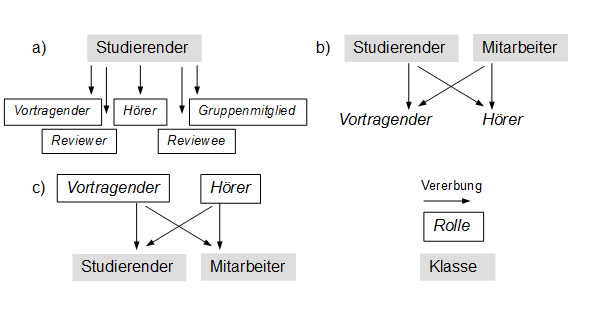
\includegraphics[scale=0.6]{Images/OomRoleProblems.PNG}
\caption{Modellierung von Rollen als Oberklasse oder Unterklasse.}
\end{figure}
%Einschränkung von relationen: intra-relationen, inter-relationen, kardinalitäten
\section{Herausforderungen und Probleme rollenbasierter Sprachen} Wie Steimann und Kühn feststellten, gibt es keine einheitliche Definition der Rolle \cite{family}\cite{steimann2000representation}. Statt einer Definition, welche immer weiter ausgarbeitet und verbessert wird, entstanden viele unterschiedliche Definitionen und Ansichten. Steimann nennt als Ursache, dass Rollen in verschiedenen Kontexten verwendet wurde und Autoren sich auf unterschiedliche Aspekte der Rollen konzentrierten \cite{steimann2000representation}. Diese Ansätze überlappen sich zwar in vielen Bereichen, aber jede neue Definition führte zu einer breiteren Zerstreuung des Begriffs oder gar zu Widersprüchen. Dies erschwert es eine, Definition zu finden, die alle Merkmale umfasst. Die Widersprüche der Ansätze müssen nicht unbedingt konzeptionell sein, dass die Merkmale zweier Definitionen einander ausschließen. Kamina und Tamais Definition\cite{kamina2005selective} eines \textit{Kontexts} unterscheidet sich stark von Deys Definition\cite{dey2001understanding}, aber wie Kühn feststellte, ließen sich beide Ansichten vereinen, indem lediglich eine neue Bezeichnung hinzugezogen wird.  \\ Möglicherweise durch diese Uneinigkeit bedingt, mangelt es rollenbasierten Modellierungs- und Programmiersprachen an Unterstützung durch Software. Dadurch sind viele Ansätze nicht ohne weiteres in der Praxis anwendbar. Außerdem wurde in nur wenigen Ansätzen, das Konzept der Rolle formal festgelegt bevor es verweundet wurde.\\ Zhu und Alkins nennen weitere Hindernisse für rollenbasierte Prgorammierung \cite{zhu2006towards}. Als größte Herausforderung nannten sie die Wahl des Abstraktionsgrades. Bevor eine neue Sprache entwickelt wird, muss klar sein, ob eine Rolle als Objekt, Klasse oder weder noch dargestellt wird. Außerdem sei eine Struktur zur Beschreibung einer Rolle notwendig. Sie soll ausdrücken können ob ein Objekt eine Rolle spielt und um welche es sich handelt. \\

Schütze und Castrillon analysierten aktuelle rollenbasierte Programmiersprachen mit Schwerpunkt auf deren Verarbeitungszeit\cite{schutze2017analyzing}.\\ Die Programmiersprachen ROP, Object Teams, LyRT und SCROLL haben einen Befehl ausgeführt im Kontext einer Bank, wodurch alle \textit{CheckingAccounts} mit allen \textit{SavingsAccounts} eine Transaktion durchführten. Im Test konnte ROP am schnellsten und in annehmbarer Zeit die 2,25 Millionen Transaktionen beenden. Object Teams war im Durchschnitt bis zu 60 mal langsamer. Dies scheint aber noch akzeptabel, im Vergleich zu LyRt und SCROLL, welche nur einen Bruchteil der Transaktionen durchführen konnten. Dabei war LyRT etwa 84.000 und SCROLL 600.000 mal langsamer als ROP. Ein weiterer Aspekt ist die Generierung von Daten während der Ausführung. Auf einer Grundlage von 250 MB produzierte ROP 365 MB an Daten und schnitt damit erneut am besten ab, während die anderen drei Sprachen Mengen von 2,8 GB bis 21,7 GB Daten generierten. Schütze und Castrillon begründen die hohe Verarbeitungszeit damit, dass die Sprachen versuchten alle Aspekte einer Rolle zu berücksichtigen. ROP ist zwar deutlich schneller und effizienter als die anderen Ansätze, leidet aber unter dem Problem der Objektschizophrenie. Jedes Mal wenn ein Objekt eine neue Rolle annimmt, wird eine Instanz des \textit{Rollenobjektes} erzeugt und zum \textit{Kernobjekt} hinzugefügt. Die Identität des Objekts wird somit aufgesplittet.
%Das \textit{Rollenobjekt} entstand durch die Nachfrage Rollen dynamisch zur Laufzeit anzunehmen \cite{baumer2000role}. Ein Objekt nimmt eine Rolle an, indem ihm ein neues Rollenobjekt hinzugefügt wird. Wie am Anfang des Kapitels beschrieben, ist die Aufsplittung der Identität des Objekts einer der größten Probleme rollenbasierter Sprachen.  \paragraph{Object Teams} \paragraph{LyRT} \paragraph{SCROLL} SCROLLING IT \\ Desweiteren 


\begin{figure}
\centering
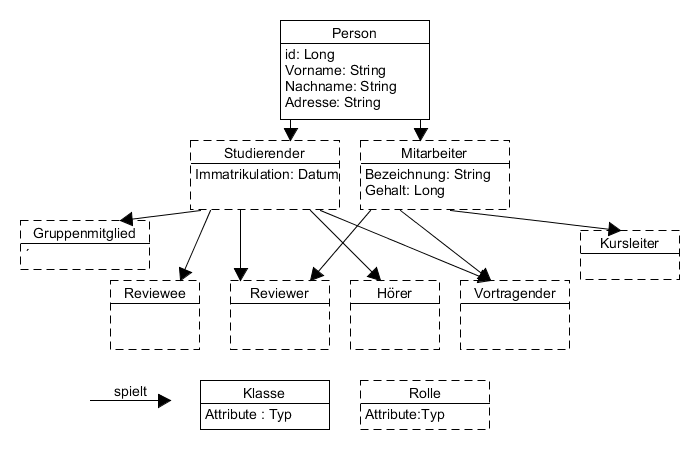
\includegraphics[scale=0.4]{Images/collabLearningBehavorial.PNG}
\caption{Die vorhandenen Rollen in einer kollaborativen Lernumgebung}
\end{figure}
%Model behavorial, relations, context
\section{Rollenbasierte kollaborative Lernumgebung}
In diesem Kapitel wird eine kollaborative Lernumgebung modelliert. Das System soll alle Szenarien, beschrieben im Kapitel 3A, darstellen können. Als Vorbild dient das informelle Modell einer Bank von Kühn \cite{family}. Es wird die Reihenfolge der umgesetzten Aspekte der Rolle übernommen. \\In Abbildung 3 sind alle Zustände, die das Verhalten einer Person beeinflussen, als Rollen zu sehen. Als natürlicher Grundtyp steht die \textit{Person}. Jeder registrierte Nutzer ist eine Instanz der Klasse Person. Als solche nehmen sie die Rolle des \textit{Studierenden} oder des \textit{Mitarbeiters} an. Es können beide Rollen gespielt werden, wenn ein Studierender sich dazu entscheidet beispielsweise als studentische Hilfskraft an der Hochschule angestellt zu sein. Durch die Zuordnung von Unterrollen wird angegeben, welche Rolle eine Person zuerst angenommen haben muss, um dessen Unterrollen spielen zu können. \\ 

Zwar sind alle Rollen enthalten, dennoch ist der kollaborative Charakter der Rollen und der Lernumgebung noch nicht ausgeprägt. Wie sich \textit{Reviewee} und \textit{Reviewer} zueinander verhalten mag intuitiv sein, aber nicht unbedingt die Interaktion zwischen einem \textit{Kursleiter} und einem \textit{Vortragenden}. Die Beziehungen zwischen den Rollen wird in Abbildung 4 ergänzt. Damit werden alle Interaktionen innerhalb der Lernumgebung im Diagramm wiedergegeben. Es werden die Menge der Beteiligten einer Beziehung angegeben, zum Beispiel, dass ein \textit{Vortragender} vor mehreren \textit{Hörer} spricht oder dass jeder \textit{Koordinator} alleine die restlichen \textit{Gruppenmitglieder} organisiert. Ein \textit{Vortragender} spricht vor mehreren \textit{Hörern} und stellt ihnen mithilfe eines ARS Systems fachbezogene Fragen, welche dann von allen beantwortet werden können.\\

Im jetzigen Zustand des Diagramms, kann jeder Reviewer nur einen Reviewee bewerten und umgekehrt. Dadurch ist noch nicht berücksichtigt, dass ein Studierender in mehreren Kursen \textit{Reviewer} sein kann und somit auch mehrere \textit{Reviewees} bewertet. In der Implementation kann dies bewerkstelligt werden, indem Rollen als eigene aber zugehörige Instanzen umgesetzt werden. In der Modellierung wird dafür ein \textit{Kontext} verwendet.Das Vorbild ist das \textit{Behälterobjekt}, beschrieben von Kühn, aus Kapitel IV c). In Abbildung 5 ist der Kontext eines \textit{Kurses} zu sehen.  Innerhalb existieren \textit{Veranstaltungen}, \textit{Ausarbeitungen}, \textit{Diskussionen} und \textit{Arbeitsgruppen}. Durch seine Behältereigenschaften werden alle Objekte und Beziehungen im \textit{Kurs} isoliert von allen anderen \textit{Kursen} betrachtet. Ein \textit{Mitarbeiter} kann also in mehreren \textit{Kursen} als \textit{Kursleiter} fungieren oder auch als \textit{Hörer} teilnehmen. Da die Rolle des \textit{Kursleiters} nur im Kontext des \textit{Kurses} betrachtet wird, werden kurzspezifische Angelegenheiten wie zum Beispiel Zugangsberechtigungen erleichtert. Zu jeder \textit{Veranstaltung} wird der \textit{Vortragende} durch den \textit{Kursleiter} bestimmt. In den meisten Fällen wird er selbst der Vortragende sein, hat aber noch die Möglichkeit die Rolle an einen Kollegen oder einen Studierenden als solchen zu bestimmen. Innerhalb einer Arbeitsgruppe können die Rollen \textit{Koordinator} und \textit{Protokollant} einmal vergeben werden. Alle anderen bleiben einfache \textit{Gruppenmitglieder}. Jede \textit{Arbeitsgruppe} wird vom Leiter des Kurses beaufsichtigt und gleichzeitig bei Bedarf konsultiert.\\ Mitarbeiter und Studierende können sich im Rahmen eines Kurses an Onlinediskussionen beteiligen. Verfassen sie in einer \textit{Diskussion} einen Beitrag, nehmen sie die Rolle des \textit{Diskussionsteilnehmer} an und werden benachrichtigt, sobald weitere Beiträge erstellt wurden. \\


\begin{figure}
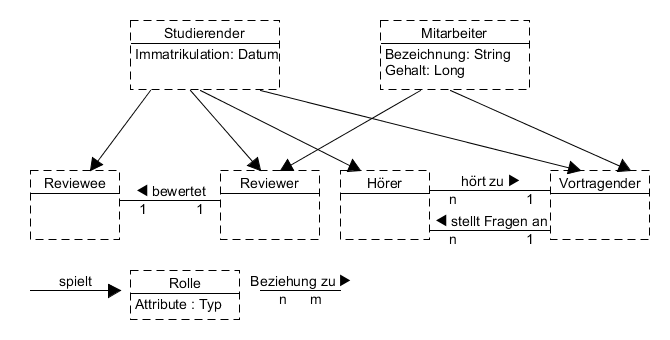
\includegraphics[scale=0.4]{Images/collabLearningRelations.PNG}
\caption{Die Interaktion zwischen Rollen in Form von Beziehungen.}
\end{figure}



\begin{figure*}
\centering
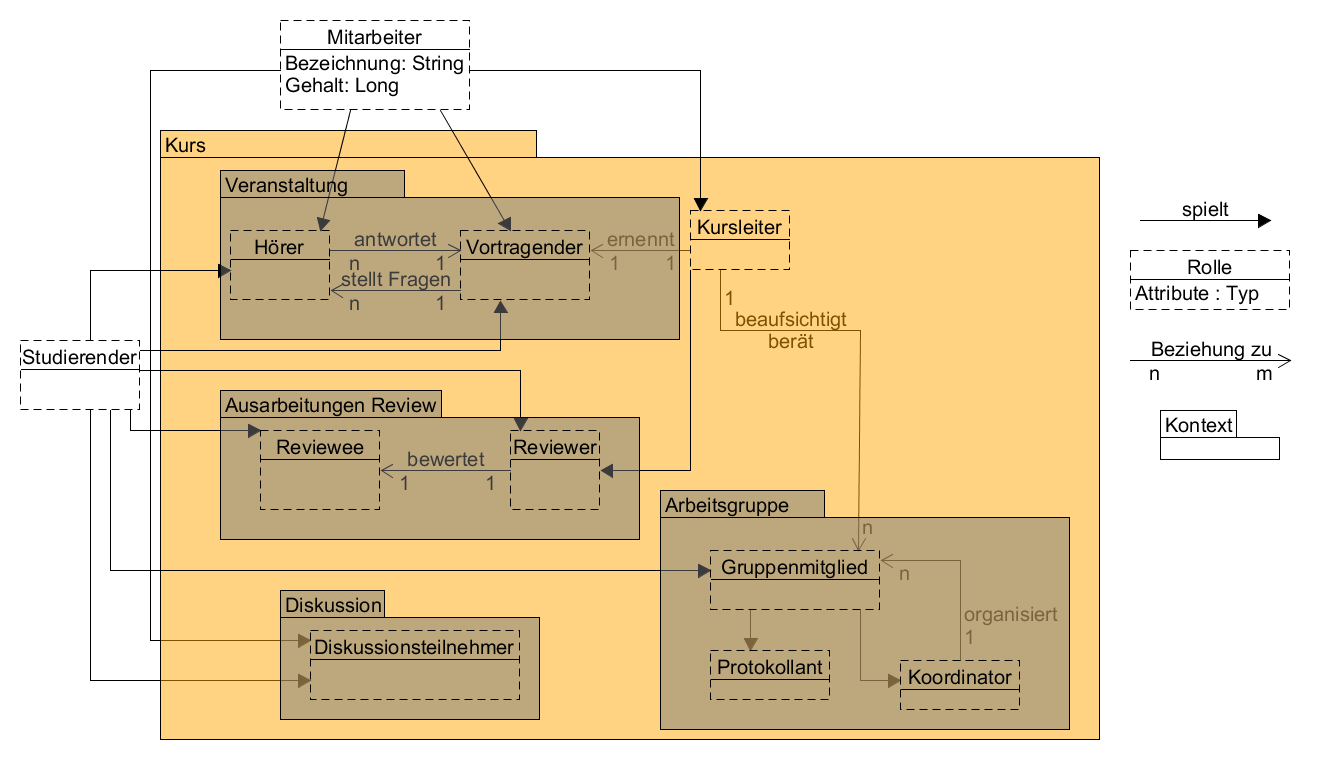
\includegraphics[scale=0.4]{Images/collabLearningContexts.PNG}
\caption{Modell zur Veranschaulichung der \textit{Kontexte}}
\end{figure*}

Das Modell umfasst nun alle Rollen, Interaktionen und Kontexte, aber gibt noch nicht alle Beziehungen und Merkmale der Rollen wieder. So lassen sich die einschränkenden Eigenschaften von Beziehungen nicht wiedergeben, ohne das Modell durch ein weiteres Pfeilsymbol unübersichtlich zu machen. Beispielsweise sind \textit{Hörer} und \textit{Vortragender} Rollen, die sich gegenseitig ausschließen, da eine Person nicht beide Rollen innerhalb einer Veranstaltung spielen kann. \\Die Beziehung \textit{bewertet} zwischen \textit{Reviewee} und \textit{Reviewer} wird momentan nicht als \textit{irreflexiv} gekennzeichnet, somit kann sich ein Studierender selbst bewerten. Desweiteren ist im Modell noch nicht verdeutlicht wie oft Rollen innerhalb eines Kontexts existieren dürfen, wie zum Beispiel, dass es nur einen \textit{Kursleiter} pro \textit{Kurs} gibt. In einer \textit{Arbeitsgruppe} ist der Aspekt der Kollaboration am stärksten gegeben. Die allgemeine gemeinsame Aufgabenbewältigung ist im Modell jedoch nicht beschrieben. Die Ursache dafür ist, dass Aufgabenstellungen und die mit der Lösung verbundenen Interaktionen sehr variabel sein können. Es lässt sich nur schwer vorhersehen, welche Rechte und Verhalten ein \textit{Gruppenmitglied} annehmen muss, um seinen eigenen Anteil der Aufgabe zu bearbeiten. Eine Lösung wäre die dynamische Erstellung einer Rolle, die im Laufe eines Kurses definiert und geändert werden kann. 


%rolle betrachtet, analysiert, probleme oom, entwurf lernumgebung, modell, diskussion
\section{Fazit}
Die jahrzehnte lange Forschung der Rolle weist, angesichts des geringen Einflusses auf moderne Computersysteme, auf ein großes unangetastes Potenzial hin. Größtes Hindernis der Rolle sind die vielen Konzepte und Sichtweisen, die aus ihrer Stärke, der Vielseitigkeit, entstanden. 
Diese Arbeit beschäftigte sich mit der Frage, inwiefern eine kollaborative Lernumgebung durch eine rollenbasierte Umsetzung besser werden könnte, als bei einer klassisch objektorientierten. Um diese Frage zu klären, wurden zunächst Anwendungsfälle in Lernumgebungen gesammelt, um eine konkrete Anwendung für das Rollenkonzept zu haben. Da eine Alternative zur Objektorientierung gesucht wird, musste zunächst ersichtlich werden, wo die Grenzen und Probleme objektorientierter Sprachen sind. Mit diesem Wissen wurde der Begriff der Rolle beleuchtet. Steimann \cite{steimann2000representation} und Kühn \cite{family} haben sich der wichtigen Aufgabe gewidmet, alle Konzepte und Facetten der Rolle zusammenzufassen. Beide Arbeiten haben einen leichten und schnellen Überblick über die verschiedenen Auffassungen der Rolle ermöglicht. Es wurden Vorteile auf konzeptioneller Ebene ersichtlich. Probleme wie multiple und dynamische Klassifikation ließen sich mit Rollenorientierung effizienter und effektiver lösen als mit Objektorientierung. Schütze stellte allerdings fest, dass moderne rollenbasierte Sprachen wesentlich langsamer arbeiten und mehr Speicherplatz in Anspruch nehmen. Dies ist teilweise darauf zurückzuführen, dass es sehr wenige Tools, die die Entwicklung rollenbasierter Anwendungen, gibt. Bei der Modellierung einer kollaborativen Lernumgebung wurde erneut deutlich, wie schwierig es ist in einem Modell, alle Aspekte der Rolle ausreichend zu berücksichtigen. \\ Es lässt sich sagen, dass rollenbasierte Programmiersprachen zunächst noch verfeinert und unterstützt werden müssen, bis sie eine lohnende Alternative zu objektorientierter Programmierung darstellen. Positivere Aussichten gibt es für die Rolle als Erweiterung der Objektorientierung. Steimann hat bereits mit der Modellierungssprache \textit{Lodwick} gezeigt, wie sich Rollen in objektorientierten Sprachen darstellen lassen. \\ Die Stärken der Rollen liegen in der Kollaboration, unvorhergesehenen Anpassungen und Vielseitigkeit. Genau deswegen sind rollenbasierte Ansätze so interessant für kollaborative Umgebungen, wo immer verschiedene Menschen zusammenarbeiten um immer verschiedene Probleme zu lösen. 
\bibliography{mybib}{}
\bibliographystyle{plain}


%to do: Hauptteil(Umsetzung der Lernumgebung in einem rollenbasiertem Modell) mit Grafik, Diskussion+fazit+future works, oom-Grafik, Zhus begründung für rollen in kollaboration
%Maybe to do: balance zwischen objektschizophrenie und statusabhängigkeit, 16+ features

\end{document}
